\section{Diagramas de atividades}
De forma a ser possível detalhar de forma simples as ações do ator nos diferentes ecrãs foram 
desenvolvidos diagramas de atividades, com isto 

\subsection{Diagrama de atividades página inicial}

Na página inicial da aplicação é possível se deslocar para o fórum, ver as notificações, realizar operações
de catálogo e deslocar-se para o perfil.

\begin{figure}[htb]
    \centering
    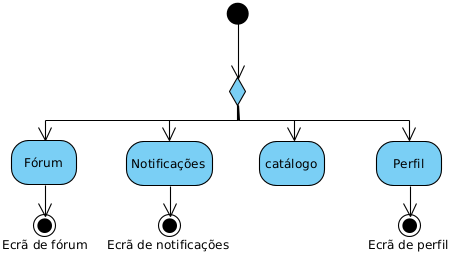
\includegraphics[width=0.6\textwidth]{images/diagramas/atividades/diagrama_atividades_home.png}
    \caption{Diagrama de atividades de página inicial da aplicação}
    \label{fig:34}
\end{figure}

\subsection{Diagrama de atividades página de perfil}

Um técnico poderá necessitar de alterar alguma configuração ou informação sua, pelo que deverá se dirigir
ao ecrã de perfil. Neste ecrã, este poderá altear a sua image de perfil, o seu nome e seu \textit{email}. 
Além disso poderá também selecionar os métodos de notificação que deseja receber e os tipos de notificação
para estes métodos. Caso uma empresa veja o seu perfil este poderá além das operações acima mencionadas
gerir os seus recursos humanos sendo encaminhada para o ecrã de gestão de recursos humanos.

\begin{figure}[htb]
    \centering
    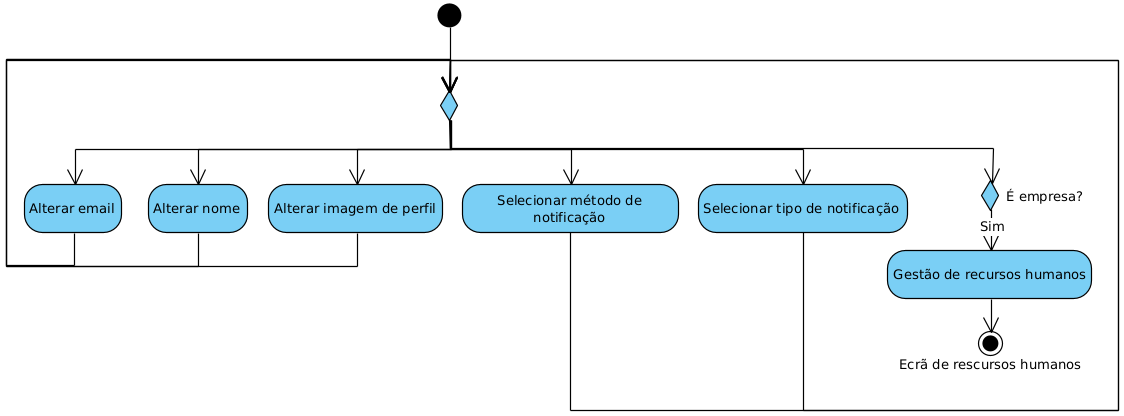
\includegraphics[width=\textwidth]{images/diagramas/atividades/diagrama_atividades_perfil.png}
    \caption{Diagrama de atividades de página de perfil}
    \label{fig:35}
\end{figure}

\newpage

\subsection{Diagrama de atividades página inicial do fórum}

Na página inicial do fórum o utilizador poderá então selecionar um dos tipos de pesquisa, escrita 
ou código QR, filtrar por tipo de tópico ou selecionar tópico. Este conseguirá também ver as 
listagens de tópicos em destaque, tópicos mais recentes e por fim tópicos por 
responder, estas listas poderão ser também filtradas por tipo, conseguindo o 
técnico depois realizar todas as ações novamente, sobre estas listas o utilizador também poderá 
selecionar um tópico o que o redirecionará para o ecrã de detalhes de tópico. Para além das 
destas operações, o técnico consegue também ver os seus tópicos e criar um novo tópico.

\begin{figure}[htb]
    \centering
    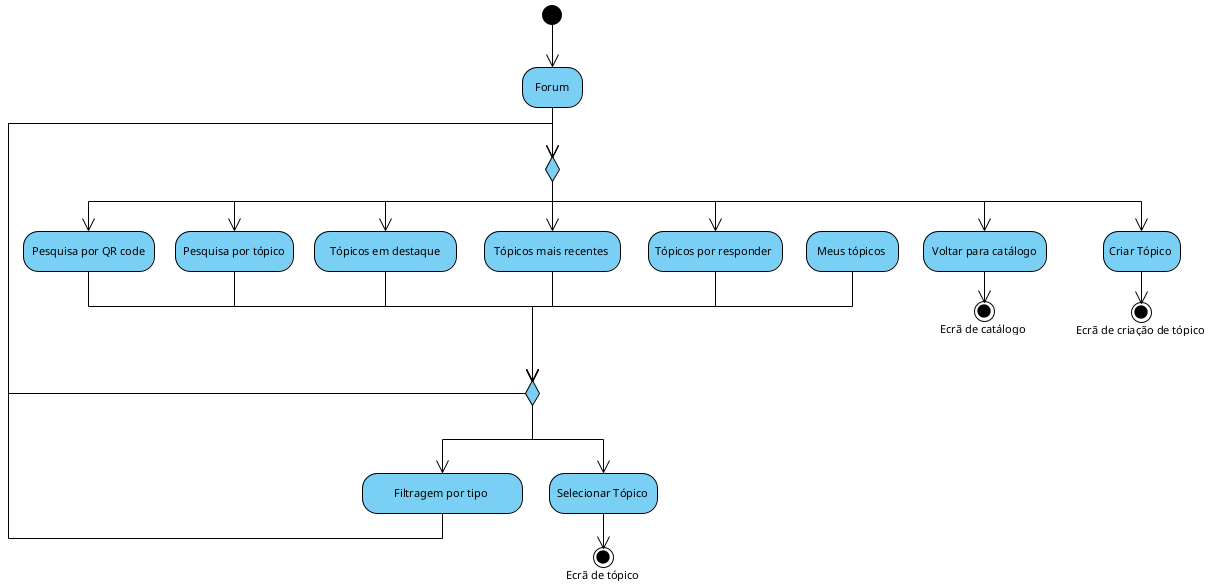
\includegraphics[width=\textwidth]{images/diagramas/atividades/diagrama_atividades_forum.png}
    \caption{Diagrama de atividades de página inicial do fórum}
    \label{fig:36}
\end{figure}



\newpage

\subsection{Diagrama de atividades página de criação de tópico}

Quando o técnico decide criar um tópico, este é encaminhado para o ecrã de criação de tópico 
onde este obrigatoriamente tem de indicar o título, descrição e tipo do tópico, por predefinição a 
visibilidade deste é pública, mas o técnico poderá alterar esta visibilidade também. 
Facultativamente o técnico poderá indicar o produto referente ao tópico, 
assim como anexar imagens, conseguindo também remover estas. A qualquer momento o técnico poderá 
confirmar a criação do tópico, quando esta ação inicia, é verificado se o título e descrição estão 
preenchidos, caso estes dados não estejam preenchidos é indicado que estes dados estão em falta, 
caso contrário este volta para o ecrã anterior.

\begin{figure}[htb]
    \centering
    \includegraphics[width=0.7\textwidth]{images/diagramas/atividades/diagrama_atividades_criar_tópico.png}
    \caption{Diagrama de atividades de página de criação de tópico}
    \label{fig:37}
\end{figure}

\newpage

\subsection{Diagrama de atividades página de detalhes do tópico}

Assim que o utilizador seleciona um tópico este é redirecionado para o ecrã de detalhes de tópico, 
no qual este poderá visualizar todas as respostas e ver as imagens anexadas em ponto grande.
Já o técnico poderá, além disso, apagar um comentário caso seja seu, gostar do tópico e de uma resposta, 
comentar, responder a um comentário. Caso o tópico seja do técnico, este poderá também alterar a 
visibilidade do tópico, marcar como concluído ou remover este voltando para o ecrã anterior. 
A qualquer momento o técnico poderá também retroceder para o ecrã anterior.

\begin{figure}[htb]
    \centering
    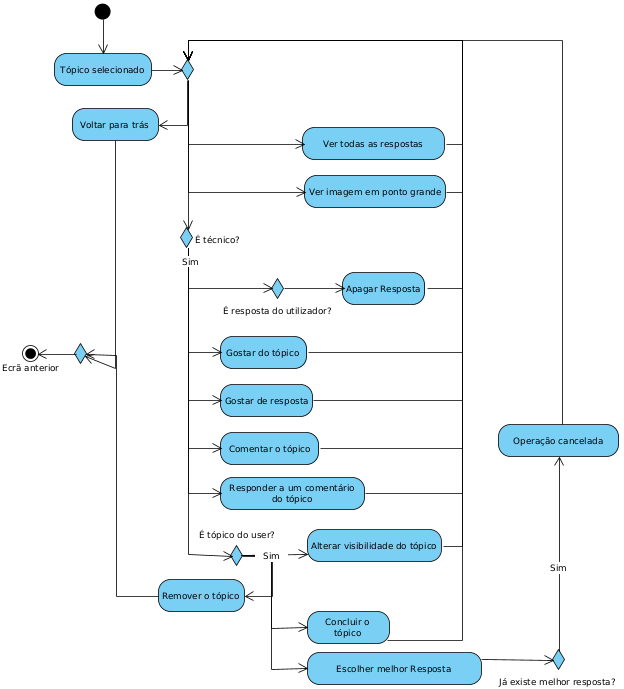
\includegraphics[width=0.9\textwidth]{images/diagramas/atividades/diagrama_atividades_detalhes_topico.png}
    \caption{Diagrama de atividades de página de detalhes do tópico}
    \label{fig:38}
\end{figure}

\newpage

\subsection{Diagrama de atividades páginas de autenticação}

Para realizar a ativação da conta de técnico, assim que este realiza o registo, confirmação de conta ou 
o login com uma conta que não se encontra ativada, este é encaminhado para o ecrã de 
ativação de conta, neste ecrã este poderá cancelar a ativação de conta, ou então indicar o código 
de ativação de conta, caso este código esteja errado, o técnico deverá inserir novamente o código, 
caso seja um código correto o técnico validará a sua conta e ficará autenticado. O técnico poderá 
também em caso de necessidade pedir o envio de um novo código de ativação de conta.

\begin{figure}[htb]
    \centering
    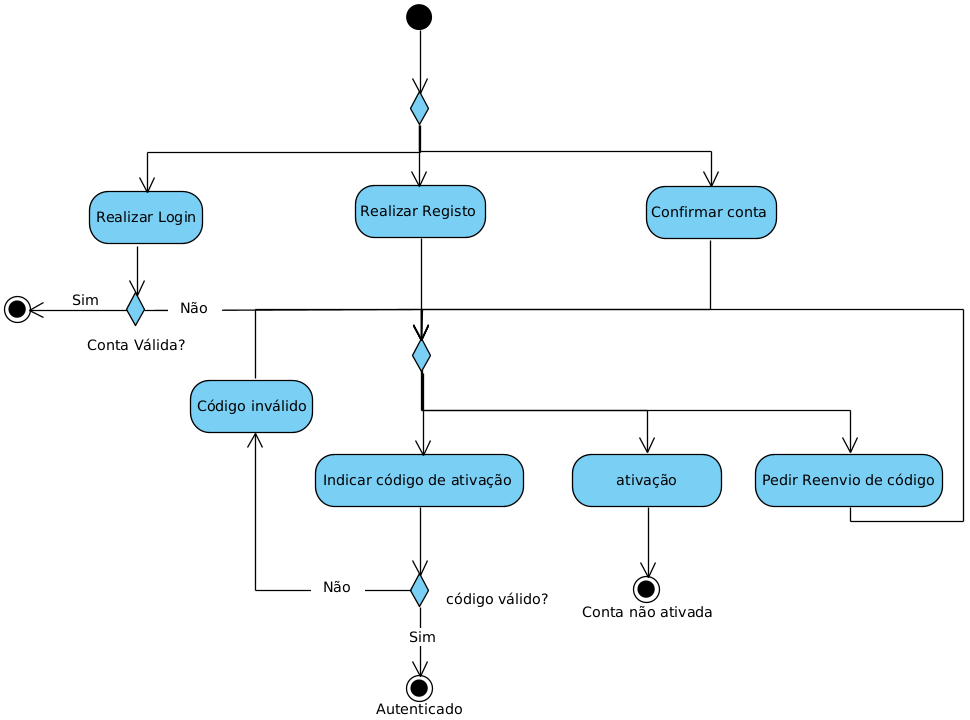
\includegraphics[width=0.8\textwidth]{images/diagramas/atividades/diagrama_atividades_autenticação.png}
    \caption{Diagrama de atividades de página de validação de conta}
    \label{fig:39}
\end{figure}

\newpage

% \subsection{Diagrama de atividades página de notificações}

% Sempre que o técnico recebe uma notificação, este poderá ver esta notificação no ecrã de notificações, 
% Este ecrã permite ao utilizador selecionar uma notificação sendo redirecionado para o tópico referente,
% caso esta esteja referente a um tópico, ou então poderá apagar a notificação.

% \begin{figure}[htb]
%     \centering
%     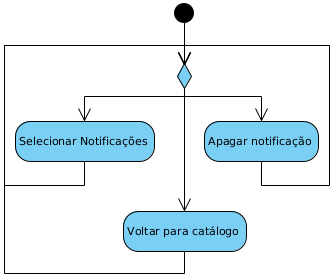
\includegraphics[width=0.5\textwidth]{images/diagramas/atividades/diagrama_atividades_noti.png}
%     \caption{Diagrama de atividades de página de notificações}
%     \label{fig:27}
% \end{figure}

% \subsection{Diagrama de atividades gestão de recursos humanos}

% Uma empresa poderá gerir as contas dos seus recursos humanos, para isso deverá se dirigir a este ecrã.
% Neste ecrã é possível registar um novo técnico sendo encaminhada para o ecrã de registo de técnico, 
% selecionar um técnico sendo encaminhada para o ecrã de perfil do técnico e poderá também pesquisar por 
% técnico.

% \begin{figure}[htb]
%     \centering
%     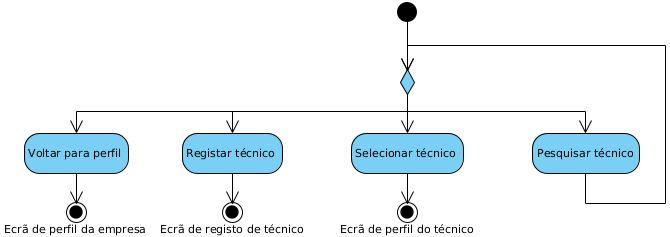
\includegraphics[width=\textwidth]{images/diagramas/atividades/diagrama_atividades_human_resources.png}
%     \caption{Diagrama de atividades de página de recursos humanos}
%     \label{fig:29}
% \end{figure}


% \subsection{Diagrama de atividades perfil de técnico}

% Sempre que uma empresa seleciona um técnico, esta é encaminhada para o ecrã de perfil de técnico. Neste 
% ecrã é possível impedir acesso à plataforma e remover a conta de técnico da plataforma.

% \begin{figure}[htb]
%     \centering
%     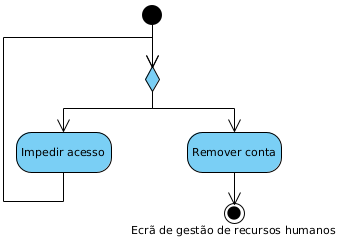
\includegraphics[width=0.5\textwidth]{images/diagramas/atividades/diagrama_atividades_prof_profile.png}
%     \caption{Diagrama de atividades de página de perfil de técnico}
%     \label{fig:30}
% \end{figure}

\newpage

\subsection{Diagrama de atividades registar técnico}

Assim que uma empresa inicia o registo de um técnico esta é redirecionada para a página de registo de técnico.
Nesta página esta terá de indicar o número de contribuinte e \textit{email} do técnico, por fim poderá confirmar o registo
de conta sendo redirecionada para a página anterior.

\begin{figure}[htb]
    \centering
    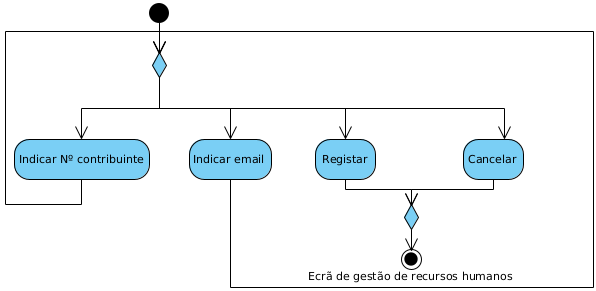
\includegraphics[width=0.8\textwidth]{images/diagramas/atividades/diagrama_atividades_add_professional.png}
    \caption{Diagrama de atividades de página de registar técnico}
    \label{fig:31}
\end{figure}

\subsection{Diagrama de atividades confirmar conta}

Quando uma conta de técnico é registada um \textit{email} de confirmação é enviado para o técnico, assim que este
recebe o \textit{email} deverá clicar em confirmar a conta sendo redirecionado para a página de confirmação de conta.
Nesta página o técnico poderá alterar o seu \textit{email}, indicar o seu nome, indicar a \textit{password} e confirmar esta, 
finalizando quando decidir se registar.

\begin{figure}[htb]
    \centering
    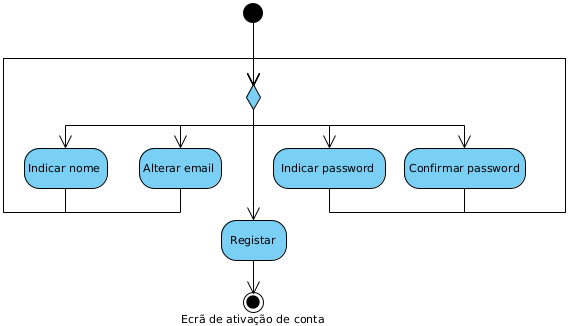
\includegraphics[width=0.8\textwidth]{images/diagramas/atividades/diagrama_atividades_prof_register.png}
    \caption{Diagrama de atividades de página de confirmar conta de técnico}
    \label{fig:31}
\end{figure}